\documentclass[11pt,a4paper]{article}

\usepackage[T1]{fontenc}
\usepackage[utf8]{inputenc}
\usepackage{lmodern}
\usepackage{microtype}
\usepackage[margin=2.6cm]{geometry}
\usepackage{booktabs}
\usepackage{graphicx}
\usepackage{amsmath}
\usepackage{caption}
\usepackage[numbers,sort&compress]{natbib}
\usepackage[hidelinks]{hyperref}

\captionsetup{font=small,labelfont=bf}
\graphicspath{{figures/}}
% generated by analysis/make_numbers.py -- do not edit

\newcommand{\AssertionsPerPair}{1.51}
\newcommand{\BinYears}{25}
\newcommand{\BooksLexMean}{24.5}
\newcommand{\BooksSemMean}{13.1}
\newcommand{\CosContrastsWith}{0.451}
\newcommand{\CosDevelopsFrom}{0.635}
\newcommand{\CosEntails}{0.598}
\newcommand{\CosExemplifies}{0.455}
\newcommand{\CosLinked}{0.432}
\newcommand{\CosLinkedDef}{0.596}
\newcommand{\CosLinkedRaw}{0.964}
\newcommand{\CosNContrastsWith}{91}
\newcommand{\CosNDevelopsFrom}{16}
\newcommand{\CosNEntails}{40}
\newcommand{\CosNExemplifies}{40}
\newcommand{\CosNOpposes}{97}
\newcommand{\CosNRequires}{237}
\newcommand{\CosNSubsumes}{33}
\newcommand{\CosNSupports}{311}
\newcommand{\CosNUnderlies}{80}
\newcommand{\CosOpposes}{0.416}
\newcommand{\CosRequires}{0.460}
\newcommand{\CosSubsumes}{0.559}
\newcommand{\CosSupports}{0.414}
\newcommand{\CosUnderlies}{0.493}
\newcommand{\CosUnlinked}{0.121}
\newcommand{\CosUnlinkedDef}{0.513}
\newcommand{\CosUnlinkedRaw}{0.931}
\newcommand{\CoverageAfter}{80.5}
\newcommand{\CoverageBefore}{64.5}
\newcommand{\CrossCategoryPct}{62}
\newcommand{\DateCheckExact}{11}
\newcommand{\DateCheckExactPct}{61}
\newcommand{\DateCheckN}{18}
\newcommand{\DateCheckWithinOne}{13}
\newcommand{\DatedById}{139}
\newcommand{\DatesRecovered}{20}
\newcommand{\DatesRefused}{38}
\newcommand{\DiachronicPassages}{73,205}
\newcommand{\FirstBenevolence}{2.89}
\newcommand{\FirstBin}{1650}
\newcommand{\FirstConscience}{18.79}
\newcommand{\FirstDuty}{44.80}
\newcommand{\FirstInterest}{92.49}
\newcommand{\FirstMoralSense}{0.00}
\newcommand{\FirstObligation}{52.02}
\newcommand{\FirstReason}{179.19}
\newcommand{\FirstSelfLove}{0.00}
\newcommand{\FirstSympathy}{7.23}
\newcommand{\FirstThePassions}{24.57}
\newcommand{\FirstUtility}{2.89}
\newcommand{\FirstVirtue}{36.13}
\newcommand{\GraphDensity}{0.036}
\newcommand{\LastBenevolence}{27.43}
\newcommand{\LastBin}{1750}
\newcommand{\LastConscience}{14.85}
\newcommand{\LastDuty}{70.55}
\newcommand{\LastInterest}{55.70}
\newcommand{\LastMoralSense}{16.26}
\newcommand{\LastObligation}{110.42}
\newcommand{\LastReason}{167.96}
\newcommand{\LastSelfLove}{15.13}
\newcommand{\LastSympathy}{10.60}
\newcommand{\LastThePassions}{47.79}
\newcommand{\LastUtility}{12.44}
\newcommand{\LastVirtue}{123.57}
\newcommand{\MaxDegree}{71}
\newcommand{\MaxPassagesPerBook}{2,674}
\newcommand{\MeanBookJaccard}{0.330}
\newcommand{\MeanDegree}{7.2}
\newcommand{\MeanJaccard}{0.165}
\newcommand{\MedianJaccard}{0.152}
\newcommand{\MedianPassagesPerBook}{341}
\newcommand{\MenAuthors}{24}
\newcommand{\MenBooks}{153}
\newcommand{\MenMedianYear}{1733}
\newcommand{\MenPassages}{73,648}
\newcommand{\Modularity}{0.41}
\newcommand{\MostAgreedJ}{0.429}
\newcommand{\MostAgreedQuery}{utility}
\newcommand{\MostDivergentJ}{0.000}
\newcommand{\MostDivergentQuery}{the passions}
\newcommand{\NAssertions}{1,099}
\newcommand{\NAuthors}{37}
\newcommand{\NBooks}{197}
\newcommand{\NCommunities}{5}
\newcommand{\NConcepts}{202}
\newcommand{\NMenAuthors}{24}
\newcommand{\NMenBooks}{156}
\newcommand{\NMenPassages}{73,648}
\newcommand{\NOcr}{72,960}
\newcommand{\NPairs}{728}
\newcommand{\NPassages}{90,975}
\newcommand{\NTxt}{18,015}
\newcommand{\NWomenAuthors}{10}
\newcommand{\NWomenBooks}{40}
\newcommand{\NWomenPassages}{14,524}
\newcommand{\NoteMinSupport}{20}
\newcommand{\PairsConflicting}{182}
\newcommand{\PairsMulti}{237}
\newcommand{\PeakBenevolence}{1725}
\newcommand{\PeakConscience}{1650}
\newcommand{\PeakDuty}{1750}
\newcommand{\PeakInterest}{1650}
\newcommand{\PeakMoralSense}{1725}
\newcommand{\PeakObligation}{1750}
\newcommand{\PeakRateBenevolence}{30.46}
\newcommand{\PeakRateConscience}{18.79}
\newcommand{\PeakRateDuty}{70.55}
\newcommand{\PeakRateInterest}{92.49}
\newcommand{\PeakRateMoralSense}{19.28}
\newcommand{\PeakRateObligation}{110.42}
\newcommand{\PeakRateReason}{179.19}
\newcommand{\PeakRateSelfLove}{16.81}
\newcommand{\PeakRateSympathy}{10.60}
\newcommand{\PeakRateThePassions}{52.30}
\newcommand{\PeakRateUtility}{12.44}
\newcommand{\PeakRateVirtue}{123.57}
\newcommand{\PeakReason}{1650}
\newcommand{\PeakSelfLove}{1725}
\newcommand{\PeakSympathy}{1750}
\newcommand{\PeakThePassions}{1725}
\newcommand{\PeakUtility}{1750}
\newcommand{\PeakVirtue}{1750}
\newcommand{\RelContrastsWith}{107}
\newcommand{\RelDevelopsFrom}{16}
\newcommand{\RelEntails}{42}
\newcommand{\RelExemplifies}{42}
\newcommand{\RelInfluences}{3}
\newcommand{\RelOpposes}{121}
\newcommand{\RelRequires}{276}
\newcommand{\RelSubsumes}{38}
\newcommand{\RelSupports}{367}
\newcommand{\RelUnderlies}{87}
\newcommand{\RetrievalK}{20}
\newcommand{\RetrievalQueries}{30}
\newcommand{\RhoBookCount}{0.64}
\newcommand{\RhoImportance}{0.18}
\newcommand{\RhoUsageDef}{0.45}
\newcommand{\StillUndated}{38}
\newcommand{\TopHub}{Virtue}
\newcommand{\TopHubDegree}{71}
\newcommand{\TopMenLean}{War}
\newcommand{\TopMenLeanRatio}{4.98}
\newcommand{\TopWomenLean}{Sacramental Remembrance}
\newcommand{\TopWomenLeanRatio}{4.64}
\newcommand{\VecConcepts}{197}
\newcommand{\VecLinked}{712}
\newcommand{\VecPairs}{19,306}
\newcommand{\WomenAuthors}{9}
\newcommand{\WomenBooks}{37}
\newcommand{\WomenMedianYear}{1708}
\newcommand{\WomenPassages}{14,433}
\newcommand{\YearMax}{1823}
\newcommand{\YearMin}{1650}


\newcommand{\concept}[1]{\textsc{#1}}
\newcommand{\rel}[1]{\textsf{#1}}

\title{Two Descriptions of the Same Shelf:\\
       a curated concept map and a dense index over \NBooks{} works of\\
       British moral philosophy, and where they disagree}

\author{Concept Atlas project}
\date{\today}

\begin{document}
\maketitle

\begin{abstract}
Concept Atlas holds \NPassages{} passages from \NBooks{} works of British moral
philosophy printed between \YearMin{} and \YearMax{}, and describes them twice
over. A curator built a map of \NConcepts{} concepts joined by \NAssertions{}
typed relations. Separately, every passage was embedded into a
2048-dimensional vector space that knows nothing of relations and records only
which words keep company with which. The two were built independently, and
comparing them is the subject of this paper.

They agree in outline and part company in instructive ways. Once the
direction every passage shares --- the subject matter itself --- is subtracted,
concepts the map joins are markedly closer in vector space than concepts it
does not (\CosLinked{} against \CosUnlinked{} mean cosine), so the curation is
not arbitrary. But the vector space cannot hear a negation: pairs the curator
marked \rel{opposes} sit at \CosOpposes{}, and pairs marked \rel{supports} at
\CosSupports{} --- indistinguishable, and both far above the unlinked
baseline. The geometry registers that two concepts belong to the same
argument and has no access to which side of it they are on, which matters in a
literature whose central disputes are oppositions. Running the comparison the
other way turns the vectors into an auditor of the ontology: the closest pairs
carrying no assertion at all are near-duplicate concepts, several at cosine
above 0.98, which are candidates for merging.

We report four further results from the same machinery. How connected a
concept is in the map tracks how many books use it ($\rho=\RhoBookCount{}$)
far more than the curator's own importance rating ($\rho=\RhoImportance{}$).
Lexical and semantic retrieval over the same corpus return largely disjoint
pages (mean Jaccard \MeanJaccard{} at $k=\RetrievalK{}$), and the vector index
draws on roughly half as many books as BM25, narrowing what a reader sees
without telling them. The vocabulary of moral sense appears from nothing and
peaks in the quarter-century beginning \PeakMoralSense{}, while the words the
period actually spent its time on --- reason, virtue, duty --- are not the ones
it is remembered for introducing. And a method for recovering publication dates
by reading imprints off the scans raised usable coverage from
\CoverageBefore\% to \CoverageAfter\% of passages, after a first attempt
produced its own cautionary result about believing digitised front matter.
\end{abstract}

\section{Introduction}

A corpus can be described by a person or by a model, and the two descriptions
are rarely compared, because they are rarely built over exactly the same text.
Here they are. Concept Atlas is a working research system over British moral
philosophy: \NBooks{} works, \NPassages{} passages, served with full-text
search, a semantic index, a concept map and a retrieval agent. Two of its
components are independent descriptions of the same shelf.

The first is the concept map. A curator, working from the books, named
\NConcepts{} concepts --- \concept{benevolence}, \concept{moral sense},
\concept{self-love}, \concept{divine law} --- gave each a definition and a set
of aliases, placed it in a three-level category tree, and asserted
\NAssertions{} relations between them, each with a type
(\rel{supports}, \rel{requires}, \rel{opposes}, \rel{contrasts\_with},
\rel{underlies}, \rel{entails}) and a strength.

The second is the vector index. Every passage was embedded with a
sentence-transformer into 2048 dimensions and stored for nearest-neighbour
search. Nothing about the concept map entered its construction. It is a
distributional object in the sense of \citet{harris1954} and
\citet{firth1957}: it knows that two passages use language the same way, and
nothing else.

Asking one to check the other is a small instance of a general question in
digital humanities, where the interesting result is usually not that a method
worked but that it disagreed with a human reading in some specific,
diagnosable way \citep{underwood2019}. We ask three things of the pair.

\begin{enumerate}
\item Does the map's adjacency correspond to proximity in the vector space
      at all, and how much?
\item Does the correspondence hold across relation types --- in particular for
      relations of opposition, where distributional methods are known to
      struggle \citep{mohammad2013,nguyen2016}?
\item Where the two disagree most sharply, what is the disagreement about?
\end{enumerate}

We also report three findings about the corpus itself that came out of the
same machinery: what the two retrieval methods do differently
(\S\ref{sec:retrieval}), how the moral vocabulary moves across the period
(\S\ref{sec:diachrony}), and what separates the books by women from the books
by men in this particular collection (\S\ref{sec:authorship}).

\section{Corpus and system}
\label{sec:corpus}

The corpus was assembled as a working library rather than a sample. It holds
\NBooks{} works by \NAuthors{} identified authors, printed between \YearMin{}
and \YearMax{}, and reaches the index in two forms: \NOcr{} passages were read
off page scans by OCR, and \NTxt{} came from typed editions. A passage is a
text block with a page and, for scanned material, a bounding box, so any
sentence quoted by the system can be traced back to a rectangle on an image.

It is not an even collection, and no analysis here pretends otherwise. The
median work contributes \MedianPassagesPerBook{} passages and the largest
contributes \MaxPassagesPerBook{}; a handful of multi-volume editions
therefore weigh as much as dozens of pamphlets. Figure~\ref{fig:corpus} shows
the distribution across time and the mix of the two text sources.

\begin{figure}[t]
  \centering
  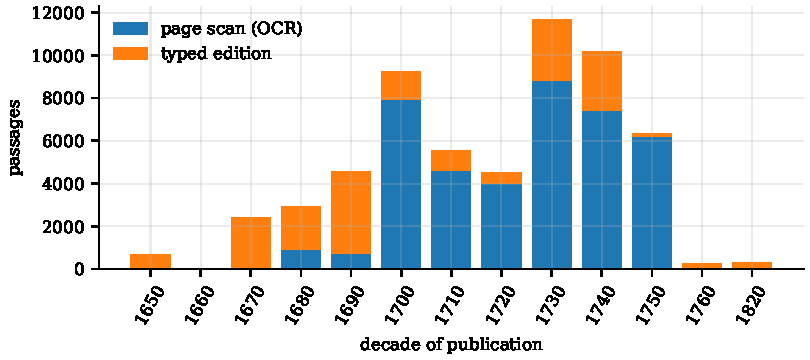
\includegraphics[width=\linewidth]{corpus_time.pdf}
  \caption{The corpus by decade of publication, split by how the text was
           obtained. The collection thickens sharply after 1700 and is
           dominated by scanned material; the typed editions are concentrated
           in the earlier period, where modern scholarly editions of women
           writers have been produced.}
  \label{fig:corpus}
\end{figure}

Two properties make the collection unusual and worth saying plainly. First,
its coverage of women writing moral philosophy is far heavier than a
conventional reading list: \WomenAuthors{} women contribute \WomenBooks{}
works and \WomenPassages{} passages, against \MenAuthors{} men with
\MenBooks{} works and \MenPassages{} passages. Second, the canonical figures
are present but not privileged; the index contains large quantities of
Rutherforth, Turnbull, Balfour and Campbell alongside Hutcheson and Hume.

Three services sit on top of the text and are used directly in what follows.
A lexical index serves BM25 \citep{robertson2009} over the OCR. A semantic
index holds every passage as a 2048-dimensional vector produced by a
sentence-transformer \citep{reimers2019}, searched by cosine on a GPU. A
retrieval agent, served by vLLM \citep{kwon2023}, calls both along with a
page-level reader, and is the component that turns a question into cited
passages. The analyses below call the same running endpoints the website
calls, so what is measured is the deployed system and not a reimplementation
of it.


\section{Reading the date off the page}
\label{sec:dates}

Any claim about change over time needs dates, and \DatedById{} of the
\NBooks{} book identifiers carry one, because they were filed as
\texttt{AUTHOR\_YEAR\_Title}. The rest --- typed editions and rescans filed
under a plain title --- carry none, and dropping them would have discarded a
third of the corpus.

Rather than supply dates from outside the collection, we read them out of it.
Title pages print the year, in arabic or roman numerals, and they sit on the
first few leaves. A first attempt simply took the earliest plausible year in
the front matter, and it failed in a way worth recording, because it is the
failure mode a digitised library invites. It dated Shaftesbury's
\emph{Characteristicks} to 1671 --- his birth year, printed in a modern
editor's note --- and gave four different works by Hutcheson the same year,
1740, because all four are reproductions of a modern edition whose preface
carries that date. Modern apparatus sits in front of the original title page
and prints dates of its own, and the naive reader cannot tell the difference
\citep{cordell2017}.

The version used here accepts a year only when the page it sits on looks like
a period title page, which in practice means an imprint line naming a place or
a printer, or when the year is set in roman numerals, which modern front
matter does not use. Any candidate equal to the author's own birth or death
year, as recorded in the project's author registry, is refused outright. That
refused \DatesRefused{} candidates and accepted \DatesRecovered{}, raising
coverage from \CoverageBefore\% to \CoverageAfter\% of passages;
\StillUndated{} works remain undated and are excluded from every analysis over
time rather than guessed at.

The method can be checked, because the books whose identifiers already carry a
year also have title pages. Running the same reader over them gives
\DateCheckN{} readable cases, of which \DateCheckExact{} match the catalogue
year exactly (\DateCheckExactPct\%) and \DateCheckWithinOne{} fall within a
year. That is a small validation set and we do not claim more from it than it
can carry: the reader is precise when it fires and fires rarely, which is the
behaviour we wanted.

One caveat governs everything downstream. What a title page prints is the year
of \emph{that impression}, not of first publication. A 1755 reprint of a 1725
argument is dated here to 1755. For the vocabulary curves in
\S\ref{sec:diachrony} this is arguably the right quantity --- it dates the
copy a reader could have held --- but it compresses the early period and must
not be read as a chronology of composition.


\section{The anatomy of a hand-built map}
\label{sec:graph}

Before comparing the map to anything, it is worth looking at what the curator
built, because its shape is not the shape one might expect from a taxonomy.

\paragraph{It is a map of support, not of division.}
The \NAssertions{} assertions fall into ten relation types, and two of them
account for more than half: \rel{supports} (\RelSupports{}) and
\rel{requires} (\RelRequires{}). Relations that separate ideas are a distinct
minority: \rel{opposes} (\RelOpposes{}) and \rel{contrasts\_with}
(\RelContrastsWith{}) together are barely a fifth of the total. The map says
far more about what holds up what than about what rules out what.

\paragraph{It says more than one thing about the same pair.}
Those \NAssertions{} assertions cover only \NPairs{} distinct pairs of
concepts, \AssertionsPerPair{} per pair. \PairsMulti{} pairs carry more than
one assertion and \PairsConflicting{} carry assertions of different kinds.
Some of these are complementary --- \rel{requires} together with
\rel{supports} is the commonest combination --- but others encode a real
tension the curator declined to resolve, such as the nine pairs marked both
\rel{contrasts\_with} and \rel{supports}, or the five marked both
\rel{opposes} and \rel{requires}. A concept pair that opposes and requires at
once is not a modelling error; it is an accurate report of a literature in
which self-love and benevolence are set against each other on one page and
made to need each other on the next.

\paragraph{It ignores its own categories.}
Each concept sits in a three-level category tree whose top level has nine
branches, the largest being Ethics (48 concepts), Moral Psychology (36),
Theology (30) and Metaphysics (30). If the categories organised the map, edges
would mostly stay inside them. They do not: \CrossCategoryPct\% of edges cross
a top-level boundary, the commonest crossings being Ethics to Moral Psychology
(84 edges) and Ethics to Theology (54). Community detection recovers
\NCommunities{} groups at modularity \Modularity{}, which is real structure
but not the category tree; the groups cut across it.

\paragraph{Its hubs are old words.}
\TopHub{} is the most connected concept by a wide margin
(\TopHubDegree{} neighbours), followed by Liberty (60), Reason (51), Habit
(49) and Providence (49). The same five top the betweenness ranking, so they
are not merely popular but load-bearing: remove them and the map falls into
pieces. What is notable is which words these are. None of the terms that
period scholarship treats as the distinctive contribution of the century ---
moral sense, sympathy, the impartial spectator --- appears near the top.
The map's skeleton is the vocabulary the century inherited, not the
vocabulary it invented.

\begin{figure}[t]
  \centering
  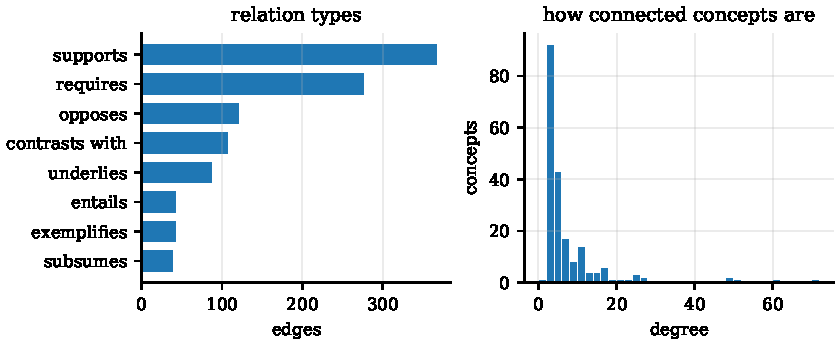
\includegraphics[width=\linewidth]{graph_anatomy.pdf}
  \caption{Left: the relation types the curator reached for, dominated by
           \rel{supports} and \rel{requires}. Right: how connected concepts
           are. The distribution is heavily skewed --- most concepts have a
           handful of neighbours and a few have dozens.}
  \label{fig:graph}
\end{figure}

\paragraph{Connection follows the books, not the curator's judgement.}
Each concept carries two curator-assigned numbers: an \emph{importance} score
and a \emph{book count} recording how many works it was found in. Degree in
the finished graph correlates strongly with book count
($\rho=\RhoBookCount{}$) and only weakly with importance
($\rho=\RhoImportance{}$). Whatever the curator meant by importance, it is not
what determined how the map got wired; textual spread is. This matters for the
next section, because it means the map is already, in part, a record of
distributional facts --- which makes the places where it \emph{departs} from
the distributional record the interesting ones.


\section{The map against the vectors}
\label{sec:vectors}

We now give every concept a second description, derived from the corpus alone.
A concept's \emph{usage vector} is the mean embedding of every passage in
which one of its aliases occurs as a whole word; \VecConcepts{} of the
\NConcepts{} concepts clear the threshold of \NoteMinSupport{} passages needed
for the mean to mean anything. Alongside it we keep the \emph{definition
vector} already used by the live query graph: the embedding of the concept's
label and the curator's gloss. The first is how the concept behaves in the
books; the second is what the curator says it is.

\paragraph{The subject matter has to be subtracted first.}
Every passage in this corpus is eighteenth-century moral philosophy, and that
shared subject is the largest single direction in the space. Left in, it
swamps everything: raw cosines between concept centroids run from 0.93 to
0.97, and pairs the map joins score \CosLinkedRaw{} against \CosUnlinkedRaw{}
for pairs it does not --- a real difference, but one three hundredths wide and
easy to mistake for noise. Subtracting the corpus mean removes the direction
every passage shares. The same comparison then reads \CosLinked{} against
\CosUnlinked{}, a gap ten times larger. Nothing about the data changed; the
common direction was simply removed from both sides. We report centred cosines
throughout, and note that any similar system which skips this step will find
that everything resembles everything.

\paragraph{The map is not arbitrary.}
Of \VecPairs{} concept pairs, \VecLinked{} are joined by at least one
assertion. Those pairs are markedly closer in the corpus than the rest
(\CosLinked{} against \CosUnlinked{}, Mann--Whitney $p<10^{-300}$), and
Figure~\ref{fig:vectors} shows the two distributions. A curator working from
the books, asserting relations by hand, produced something a distributional
model independently agrees with. The usage and definition descriptions agree
with each other more weakly ($\rho=\RhoUsageDef{}$), which is what one would
expect: a definition is written to distinguish a concept from its neighbours,
while usage records that they appear in the same paragraphs.

\begin{figure}[t]
  \centering
  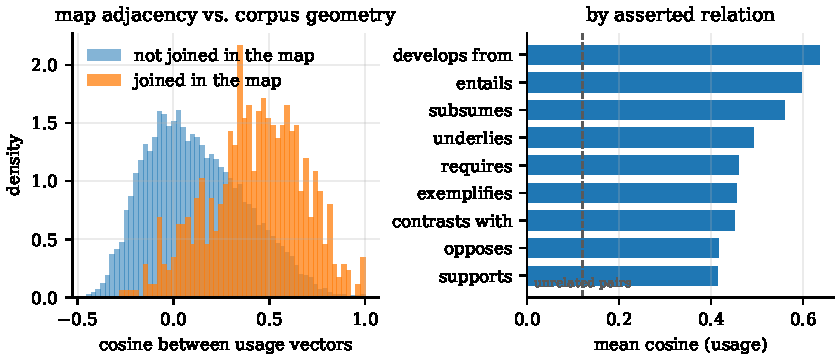
\includegraphics[width=\linewidth]{map_vs_vectors.pdf}
  \caption{Left: centred cosine between concept usage vectors, for pairs the
           map joins and pairs it does not. Right: mean cosine by the kind of
           relation asserted, against the unlinked baseline (dashed). The
           relations that order concepts hierarchically sit highest; the
           relations that set concepts against each other sit at the bottom,
           level with \rel{supports}.}
  \label{fig:vectors}
\end{figure}

\paragraph{The geometry cannot hear a negation.}
The right panel of Figure~\ref{fig:vectors} is the substantive result. Sort
the relation types by how close their pairs sit, and the order is
\rel{develops\_from} (\CosDevelopsFrom{}), \rel{entails} (\CosEntails{}),
\rel{subsumes} (\CosSubsumes{}), \rel{underlies} (\CosUnderlies{}),
\rel{requires} (\CosRequires{}), then \rel{contrasts\_with}
(\CosContrastsWith{}), \rel{opposes} (\CosOpposes{}) and \rel{supports}
(\CosSupports{}).

Two things follow. The first is that relations which arrange concepts in a
hierarchy --- one develops from another, entails it, subsumes it --- are the
ones the vector space reproduces most strongly, which makes sense: a concept
that subsumes another is discussed wherever the other is.

The second is sharper. \rel{opposes} scores \CosOpposes{} and \rel{supports}
scores \CosSupports{}. They are indistinguishable. A pair of concepts the
curator marked as standing against each other sits exactly as close, in the
corpus, as a pair marked as holding each other up --- and both sit some three
and a half standard deviations above the unlinked baseline. The geometry
registers that two concepts belong to the same argument; it has no access
whatever to which side of it they are on. This is the antonymy problem
\citep{mohammad2013,nguyen2016} arriving in a corpus where it does real damage,
because the century's central disputes are precisely oppositions: self-love
against benevolence, interest against duty, reason against sentiment. A
semantic search for evidence that an author held a position will return, with
equal confidence, the passage in which a rival denies it. The system's
verification tool, which re-reads the retrieved page before a claim is made,
exists for this reason; here is the measurement that justifies it.

\paragraph{Where the vectors correct the map.}
The pairs that sit closest in the corpus while carrying no assertion at all
are almost entirely a single kind of thing: near-duplicate concepts.
\concept{Lipsius Citation} and \concept{Seneca} have a cosine of 1.000,
meaning their aliases select identical passages. \concept{Seneca} and
\concept{Seneca Reference}, \concept{Fitness} and \concept{Moral Fitness},
\concept{Atheism} and \concept{Virtue and Atheism}, \concept{Evil} and
\concept{Origin of Evil}, \concept{Sacrament} and \concept{Sacramental
Remembrance} --- all above 0.98, none joined by an edge. The vector space is
acting here as an auditor of the ontology, and what it reports is that the map
contains a dozen concepts that are variants of another concept rather than
concepts in their own right. This is the single most directly actionable
result in the paper: these pairs are candidates for merging.

\paragraph{Where the map outruns the corpus.}
The reverse list --- pairs the map joins that the corpus places furthest apart
--- reads differently. \concept{Moral Fitness} \rel{supports}
\concept{Trinity} at $-0.26$, \concept{Sacrament} \rel{requires}
\concept{Virtue} at $-0.23$, \concept{Reason} \rel{requires}
\concept{Sacrament} at $-0.20$. These are not obviously wrong as claims about
the period; they are claims whose two halves live in different books, one
theological and one ethical, and which therefore have no shared context for a
distributional method to find. They are the assertions a reader of the whole
library can make and a model trained on passage co-occurrence cannot. Whether
they are insights or overreach is not something the geometry can settle, and
we do not pretend otherwise --- but they are exactly the list a curator should
be handed when asked to defend the map.


\section{Two retrievals over one corpus}
\label{sec:retrieval}

The site offers two ways to find a passage, and they are built to different
units. BM25 \citep{robertson2009} indexes the OCR and returns a page with a
match count. The Jasper index returns an individual text block inside a page.
A page is the finest thing both can name, and it is also what a reader follows
when they click a result, so the comparison is made at page level over
\RetrievalQueries{} queries drawn from the period's own vocabulary, asking the
running services for the top \RetrievalK{} of each.

The two agree far less than one would guess. Mean Jaccard overlap is
\MeanJaccard{} and the median \MedianJaccard{}: of twenty pages returned, three
or so are common to both lists. The most agreed query is
`\MostAgreedQuery{}' at \MostAgreedJ{}, and `\MostDivergentQuery{}' produces
no overlap at all. Figure~\ref{fig:retrieval} shows the full ranking.

\begin{figure}[t]
  \centering
  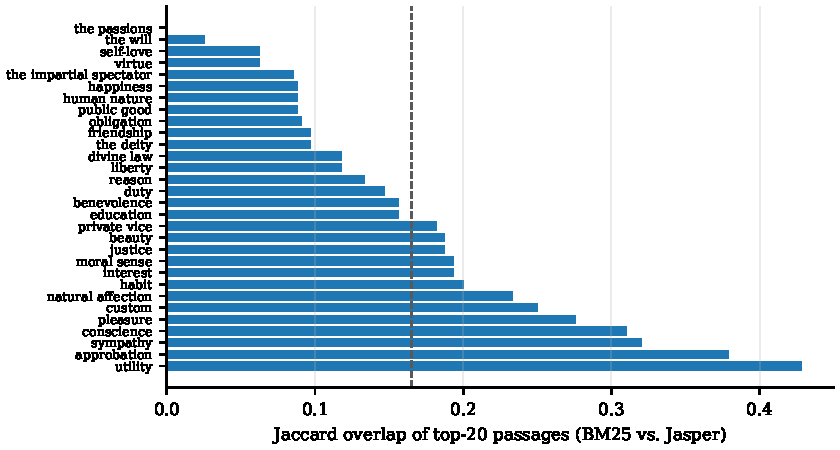
\includegraphics[width=0.94\linewidth]{retrieval_divergence.pdf}
  \caption{Overlap between BM25 and semantic retrieval for the same query, at
           page level, top \RetrievalK{}. The dashed line is the mean. Terms
           whose eighteenth-century use is close to their modern use agree
           most; terms that were technical vocabulary then agree least.}
  \label{fig:retrieval}
\end{figure}

The pattern in that ranking is not random. The queries where the two methods
agree best are the ones whose sense has changed least --- \emph{approbation},
\emph{pleasure}, \emph{custom}. The ones where they diverge most are either
very common words that BM25 matches everywhere while the vectors chase a
particular sense (\emph{the passions}, \emph{the will}, \emph{reason}), or
phrases whose period meaning is carried by surrounding argument rather than
the phrase itself.

A second difference is easier to miss and matters more for a reader. Across
the same queries, BM25 draws its top \RetrievalK{} from \BooksLexMean{}
distinct books on average; the semantic index draws from \BooksSemMean{} ---
roughly half as many. The vector index concentrates. It finds the books that
discuss a topic at length and returns several passages from each, where the
lexical index spreads thinly across everything that happens to use the word.
Neither behaviour is wrong, but a scholar who uses only the semantic index
will systematically see a narrower slice of the library, and will not be told
so. The system's hybrid default, which blends both, exists for this reason;
this measurement is the first quantification of what it is blending.


\section{A vocabulary in motion}
\label{sec:diachrony}

With dates for \DiachronicPassages{} passages, the corpus can be asked whether
it shows the story the period is usually told as: the moral sense of Hutcheson
giving way to sympathy, and sympathy in turn to the calculating language of
utility and interest. We count the share of passages in each quarter-century
that use each term --- rates, not counts, since the corpus is wildly uneven
across time and raw counts would only redraw Figure~\ref{fig:corpus}.

\begin{figure}[t]
  \centering
  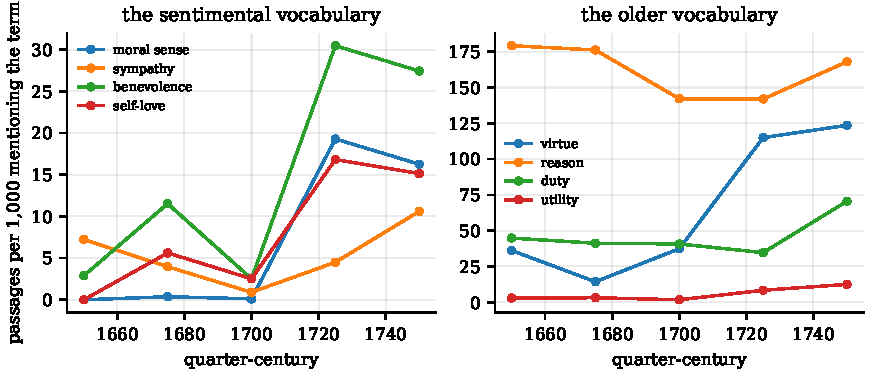
\includegraphics[width=\linewidth]{diachrony.pdf}
  \caption{Term use per 1,000 dated passages by quarter-century. Left: the
           vocabulary of moral sentiment, absent before 1700 and arriving
           together. Right: the older vocabulary, present throughout.}
  \label{fig:diachrony}
\end{figure}

The first half of the story is visibly there, and sharply. \emph{Moral sense}
does not occur at all in the first two bins --- a rate of \FirstMoralSense{}
per thousand --- and peaks in the bin beginning \PeakMoralSense{} at
\PeakRateMoralSense{}. \emph{Self-love} does the same thing on the same
schedule, from \FirstSelfLove{} to a peak of \PeakRateSelfLove{}, and
\emph{benevolence} rises from \FirstBenevolence{} to \PeakRateBenevolence{}.
These three arrive together, in the quarter-century that contains Hutcheson's
\emph{Inquiry} and \emph{Essay} \citep{hutcheson1725,hutcheson1728} and
Butler's \emph{Sermons} \citep{butler1726}. A vocabulary appears from nothing
and takes over a literature inside twenty-five years.

The second half of the story is not there, at least not here.
\emph{Sympathy} rises only modestly, from \FirstSympathy{} to
\LastSympathy{}, and never approaches the prominence of the moral-sense
cluster. \emph{Utility} likewise ends at \LastUtility{}. The obvious
explanation is the corpus rather than the period: it thins after 1750, and the
works that would carry the sympathy story --- Hume's \emph{Treatise}
\citep{hume1740} and Smith's \emph{Theory of Moral Sentiments}
\citep{smith1759} --- are represented thinly, a gap the retrieval agent
discovered independently and reported unprompted when asked to compare the two
(\S\ref{sec:limits}).

The unglamorous terms are the ones that dominate throughout. \emph{Reason}
runs at \FirstReason{} per thousand in the earliest bin and
\LastReason{} in the latest, an order of magnitude above anything in the
sentimental cluster, and declines only gently. \emph{Virtue} more than
triples, from \FirstVirtue{} to \LastVirtue{}. \emph{Obligation} and
\emph{duty} both rise substantially. Whatever else happened to British moral
philosophy across this period, the words it spent most of its time using were
not the ones it is remembered for introducing --- a result consistent with
what \S\ref{sec:graph} found in the map's hubs, arrived at by a completely
different route.


\section{Two collections}
\label{sec:authorship}

The corpus contains \WomenBooks{} works by \WomenAuthors{} women and
\MenBooks{} works by \MenAuthors{} men, which makes a comparison possible that
most eighteenth-century collections cannot support. We ask a narrow question
--- which concepts are used at noticeably different rates in the two sets ---
and take care to claim nothing wider than the answer allows.

The confounds come first, because they are large. The two sets differ in size
by a factor of five (\MenPassages{} passages against \WomenPassages{}). They
differ in date: the median dated passage by a woman is from
\WomenMedianYear{}, by a man from \MenMedianYear{}, a full generation apart.
And they differ in genre, because what survives and has been edited is not the
same for both: the women here are represented largely by devotional treatises,
letters and educational writing, the men substantially by natural-law
jurisprudence and academic moral philosophy. Any difference found below is a
difference between two \emph{collections}, produced by all three of those
factors at once. It is not evidence about authorship as such, and we do not
offer it as any.

\begin{figure}[t]
  \centering
  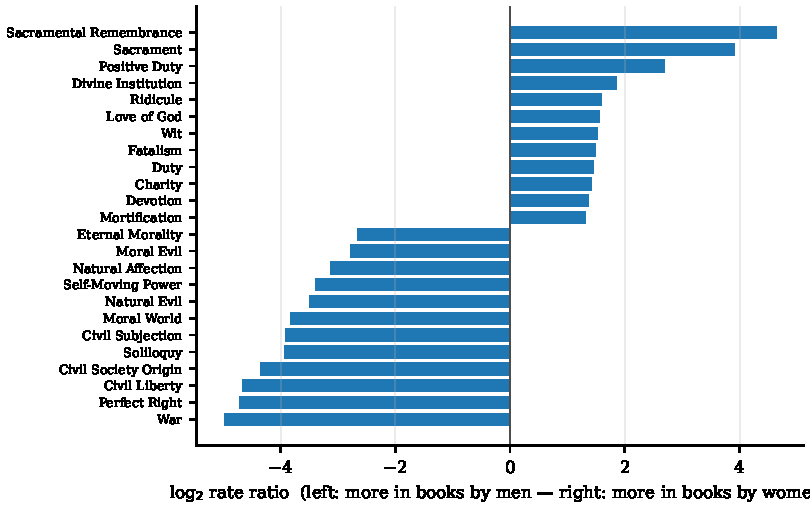
\includegraphics[width=0.92\linewidth]{authorship.pdf}
  \caption{Concepts with the most unequal rates between the two sets of books,
           as a log ratio. Only concepts appearing in at least five books on
           the leaning side are shown, so no single volume can produce an
           entry.}
  \label{fig:authorship}
\end{figure}

With that said, the separation is stark and clean. The concepts most
characteristic of the women's books are sacramental and devotional:
\concept{\TopWomenLean{}} leads at \TopWomenLeanRatio{} on a log$_2$ scale,
followed by \concept{Sacrament}, \concept{Positive Duty}, \concept{Divine
Institution} and \concept{Love of God}. The concepts most characteristic of
the men's books are political and juridical: \concept{\TopMenLean{}} at
$-\TopMenLeanRatio{}$, with \concept{Perfect Right}, \concept{Civil Liberty},
\concept{Civil Society Origin} and \concept{Civil Subjection} behind it.

Read carefully, this is a result about the shape of a discipline's archive
rather than about its authors. Moral philosophy in this period is written in
both registers --- the devotional and the juridical --- and the archive has
sorted them by the sex of the writer, because the institutional settings that
produced natural-law jurisprudence were closed to women and the devotional
tradition was not. The measurement recovers that sorting with considerable
precision. What it cannot do, and what no count of aliases could do, is
distinguish a writer choosing a register from a writer permitted only one.


\section{Limitations}
\label{sec:limits}

\paragraph{The text is read by a machine and is imperfect.}
\NOcr{} of the passages come from OCR of period printing, with long
\textit{s}, broken type and catchwords. Dirty OCR does not corrupt these
results evenly: it suppresses rare strings more than common ones
\citep{cordell2017}, which means every rate reported in
\S\ref{sec:diachrony} is a lower bound, and the rarer the term the more it is
depressed.

\paragraph{The collection is not a sample of anything.}
It was assembled, not drawn. Conclusions of the form ``the period did X'' are
not available from it; conclusions of the form ``this library does X'' are.
The corpus thins after 1750, so the later bins rest on less evidence than the
earlier ones, and the mid-century weight of Rutherforth, Turnbull and Balfour
reflects what was scanned rather than what was read at the time.

\paragraph{Dates are impressions, not compositions.}
As \S\ref{sec:dates} sets out, a recovered date is the year of the copy, not
of first publication. The effect is to push arguments later than their first
appearance, compressing the early period.

\paragraph{Concept occurrence is alias matching.}
A concept counts as present in a passage when one of its curator-supplied
aliases occurs there as a whole word. This misses paraphrase entirely and
catches homonyms indiscriminately --- the map's own note on
\concept{affection} warns that Rutherforth's ``affections'' are attributes of
God and a different sense of the word, and nothing here distinguishes them.
The usage vectors of \S\ref{sec:vectors} inherit this.

\paragraph{The vector space is one model's opinion.}
Every geometric claim is relative to one embedding model. A different encoder
would move the numbers; we would expect the \emph{direction} of the opposition
result to survive, since it follows from the distributional hypothesis rather
than from any particular implementation of it, but that is a prediction, not a
finding.

\paragraph{One gap the system found itself.}
Asked to compare Hutcheson's moral sense with Hume's sympathy and Smith's
impartial spectator, the retrieval agent ran 29 searches and then reported,
without being asked to check, that the index held ``limited direct text from
Smith's \emph{Theory of Moral Sentiments}, primarily editorial apparatus and
textual variants''. That is correct, and it is a real hole in the
collection rather than a failure of retrieval. It is recorded here partly as a
limitation and partly as evidence about the architecture: a retrieval agent
with a verification tool will sometimes tell you that the thing you asked
about is not in the library, which is the single most useful thing it can say
and the one a similarity ranking can never say, because a ranking always
returns its best twenty.


\section{Reproducing this}
\label{sec:repro}

Everything in this paper is generated. The analyses live in
\texttt{paper/analysis/}; they write results as JSON into
\texttt{paper/data/} and figures into \texttt{paper/figures/}, and
\texttt{make\_numbers.py} turns that JSON into the LaTeX macros the prose
uses. No number in the text was typed by hand; re-running the
analysis rewrites the paper's numbers along with its figures.

\begin{verbatim}
make -C paper analysis   # recompute everything from the corpus
make -C paper            # build paper.pdf
make -C paper check      # fail on any LaTeX warning or bad box
\end{verbatim}

Two analyses call the live services (\texttt{/bm25}, \texttt{/semantic}) and
need them running; the rest read the index files directly. The concept-to-
passage index is expensive to build and is cached in
\texttt{paper/data/concept\_support.json}, rebuilt with
\texttt{a\_support.py --force}.

The \texttt{check} target is the reason the build is worth automating. It
fails on any LaTeX warning, any overfull or underfull box, any missing
character and any unresolved reference --- the class of defect that otherwise
ships silently in a PDF.


\bibliographystyle{plainnat}
\bibliography{refs}

\end{document}
